\chapter{Problem Analysis}\label{sec_problem_analysis}
For this report, Aalborg University has made a robot with a conveyor belt available and have a demo assembly, a picture of the test setup is shown on figure \ref{fig_pic_test_setup}.
\begin{figure}[htbp]
\centering
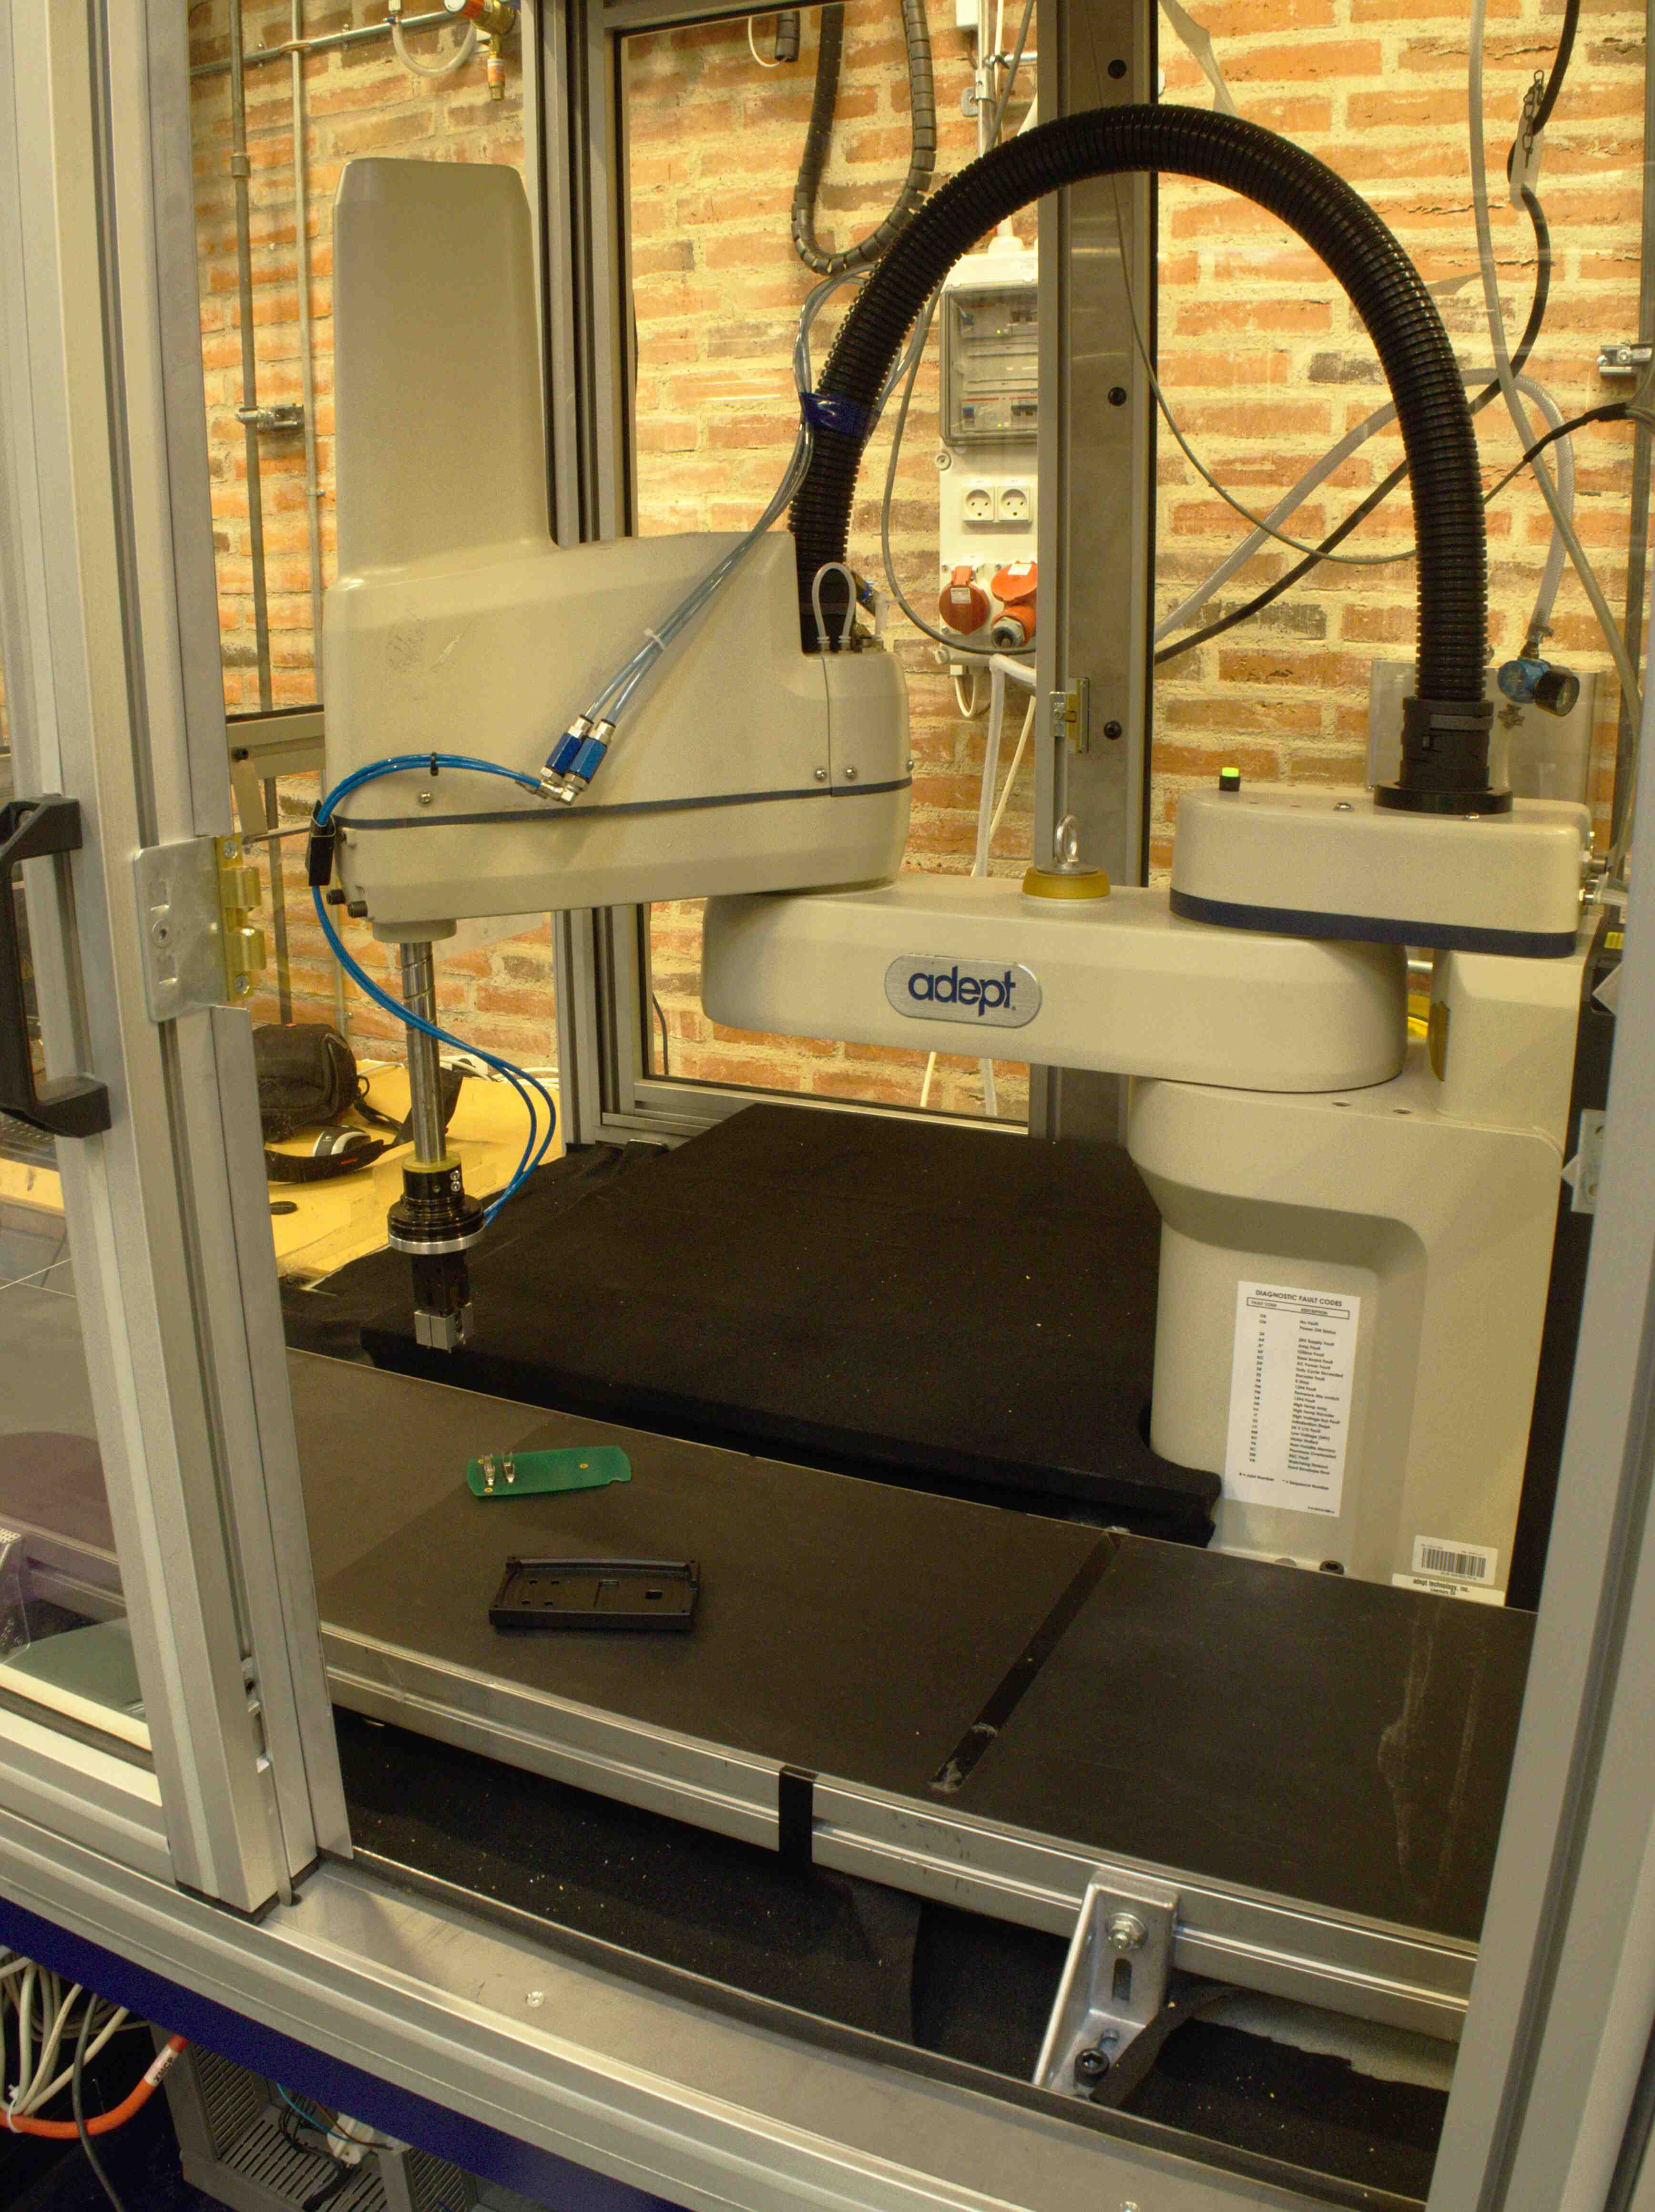
\includegraphics[width=0.5\textwidth]{prob_ana_opstilling}
\caption{The test setup made available by Aalborg University}
\label{fig_pic_test_setup}
\end{figure}\newline
The University's desire is to design a visual system for the robot, which enables it to assemble the demo assembly without any information about the conveyor belt's velocity or position. Likewise the solution needs to be efficient, which means the robot needs to pick up the parts for the assembly while the conveyor belt is moving. The purpose of this chapter is to present the assembly, test setup and analysing which modifications are necessary before the robot is able to assemble the assembly. This leads to the solution strategy for the remainder of the report. 
